% !TEX TS-program = XeLaTeX

% STYLE

\documentclass[a4paper, 12pt]{article}
\usepackage[left=1in,
		    right=1in,
    		    top=1in,
		    bottom=1in,
		    bindingoffset=0cm]{geometry}
		    \usepackage{array}
\usepackage{float}
\usepackage{graphicx}
\graphicspath{ {./images/} }
\usepackage{subfig}
\usepackage{enumerate}
\usepackage[normalem]{ulem} % underlining
\usepackage{booktabs} % tables
\usepackage[table]{xcolor} % coloring tables
\newcolumntype{L}[1]{>{\raggedright\let\newline\\\arraybackslash\hspace{0pt}}m{#1}} % beautiful column types
\newcolumntype{C}[1]{>{\centering\let\newline\\\arraybackslash\hspace{0pt}}m{#1}}

% LANGUAGE + FONT
		    
\usepackage[english]{babel}
\usepackage[backend=biber,
                     style=unified]{biblatex}
\newcommand{\citeay}[2][]{
   \citeauthor{#2} (\citeyear[#1]{#2})}
\addbibresource{ref.bib}
\usepackage{fontspec}  
\setmainfont{Minion 3}

% DRAWING

\usepackage{tikz}
\usepackage{tikz-qtree}
\usetikzlibrary{shapes.geometric}
\usetikzlibrary{trees,arrows}
\usetikzlibrary{positioning}
\usetikzlibrary{matrix}
\usetikzlibrary{tikzmark}
\usetikzlibrary{decorations.shapes}

% LINGUISTICS 

\usepackage{expex}
\usepackage[glossaries]{leipzig}
\makeglossaries
\newleipzig {npst} {npst} {non-past}
\newleipzig {nfin} {nfin} {non-finite}
\newleipzig {nsg} {nsg} {non-singular}

\lingset{numoffset=1ex, aboveexskip=1em, belowexskip=1em}

\title{Estonian dataset}
\author{EGG2023, Novi Sad}
\date{Last updated \today}

\begin{document}
\maketitle

	\section{Basic facts}
	
	Consonant and vowel inventories \parencite{asu-teras2009}
	
	\begin{figure}[H]
		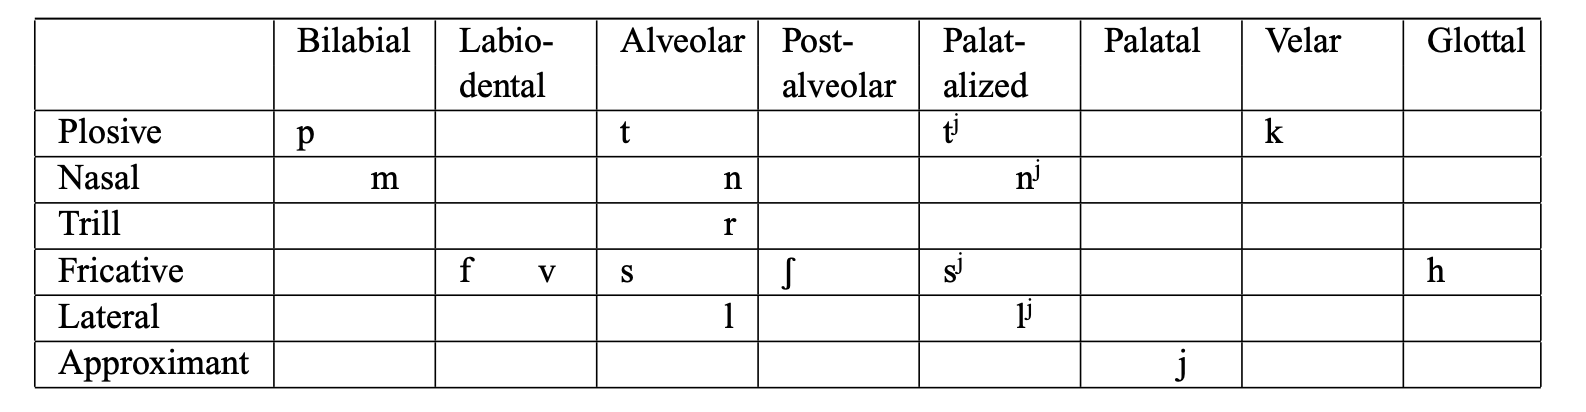
\includegraphics[scale=.6]{est-consonants}
	\end{figure}
		
	\begin{figure}[H]
		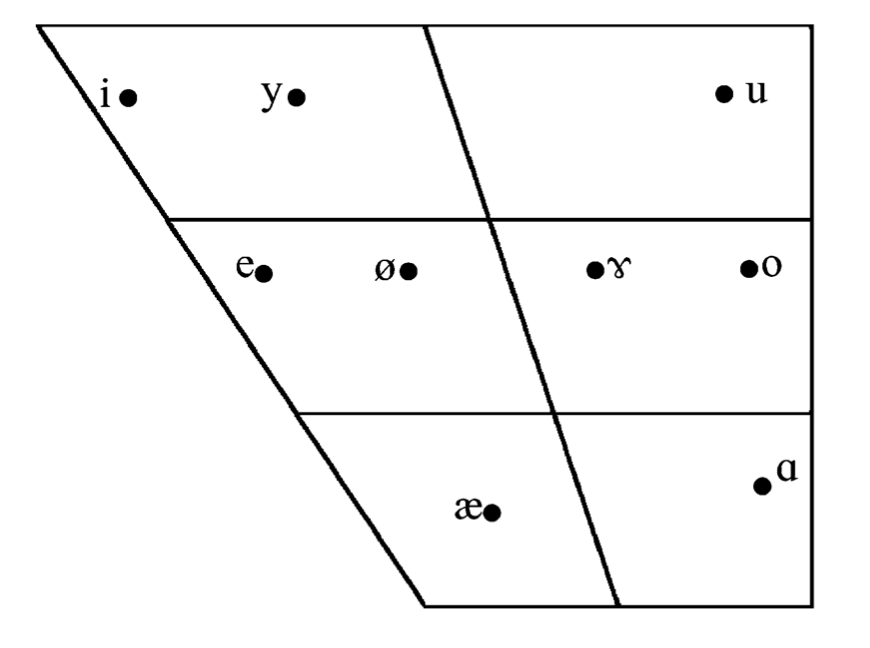
\includegraphics[scale=.5]{est-vowels}
	\end{figure}

	\section{Consonant gradation data}
	
	Several verbs in 5 different forms \parencite{problems}.

\begin{table}[H]
\begin{tabular}{llllll}
\toprule
\textbf{Infinitive I} & \textbf{Infinitive II} & \textbf{Present tense} & \textbf{Past tense} & \textbf{Participle} & \textbf{Translation} \\
\midrule
hakkama               & hakata                 & hakkan                 & hakkasin            & hakatud             & begin                \\
\addlinespace[0.2cm]
hüppama               & hüpata                 & hüppan                 & hüppasin            & hüpatud             & jump                 \\
\addlinespace[0.2cm]
näitama               & näidata                & näitan                 & näitasin            & näidatud            & show                 \\
\addlinespace[0.2cm]
kompima               & kompida                & kombin                 & kompisin            & kombitud            & feel, touch          \\
\addlinespace[0.2cm]
lõikama               & lõigata                & lõikan                 & lõikasin            & lõigatud            & cut                  \\
\addlinespace[0.2cm]
õppima                & õppida                 & õpin                   & õppisin             & õpitud              & study, learn         \\
\addlinespace[0.2cm]
põdema                & põdeda                 & põen                   & põdesin             & põetud              & be sick              \\
\addlinespace[0.2cm]
pumpama               & pumbata                & pumpan                 & pumpasin            & pumbatud            & pump                 \\
\addlinespace[0.2cm]
sulgema               & sulgeda                & sulen                  & sulgesin            & suletud             & close                \\
\addlinespace[0.2cm]
rääkima               & rääkida                & räägin                 & rääkisin            & räägitud            & speak                \\
\addlinespace[0.2cm]
tõlkima               & tõlkida                & tõlgin                 & tõlkisin            & tõlgitud            & translate           \\
\bottomrule
\end{tabular}
\end{table}

	\section{Questions to consider}
	
\begin{enumerate}[$\gg$]
	\item What are the rules that produce each form?
	\item Which of the forms is the most ``basic'' one, from which all the other are produced? 
	\item How many consonant grades grades does Estonian have?
\end{enumerate}

\printbibliography

\end{document}